% Marco Metodologico
\chapter{Marco Metodol'ogico} \label{chap:metodologia}
Para el desarrollo de un buen software es necesario la utilizaci'on de una metodolog'ia, ya que la misma brinda una serie de mecanismos y fases para el desarrollo organizado del m'odulo.
\newline
\newline
Para este proyecto, se decidi'o utilizar la metodolog'ia \textbf{ASAP (Ascendant SAP)}, ya que es la m'as utilizada para el desarrollo de aplicaciones en SAP ERP.
\section{Descripci'on de la metodolog'ia}
Seg'un Khan (2002), \textbf{ASAP (Ascendant SAP o Accelerated SAP como tambi'en se le conoce)} es una metodolog'ia que fue dise\~nada por SAP para agilizar el desarrollo de sus aplicaciones, ya que con otras metodolog'ias, un desarrollo se pod'ia llevar mucho m'as tiempo del esperado. Mientras un proyecto usando la metolodog'ia convencional se puede llevar dos a\~nos o m'as en realizarse, el mismo proyecto bas'andose en la metodolog'ia \textbf{ASAP}, puede ser realizado en menos de un a\~no. 

\section{Caracter'isticas Principales}
Seg'un Khan (2002), ASAP ha sido dise\~nado con el objetivo de estandarizar y de llevar de una forma coordinada una implementaci'on SAP.  Esta metodolog'ia posee las siguientes caracter'isticas:
\begin{enumerate}
\item Es capaz de optimizar tiempo, calidad y recursos.
\item Es capaz de aprovechar las mejores pr'acticas del negocio.
\item Es capaz de entregar un proceso orientado a un mapa de proyecto (Hoja de Ruta ASAP). Una hoja de ruta ASAP es un gr'afico que presenta los pasos o fases a seguir, como se muestra en la figura ~\ref{fig:roadmap}.

\end{enumerate}


\begin{figure}[H]
\centering
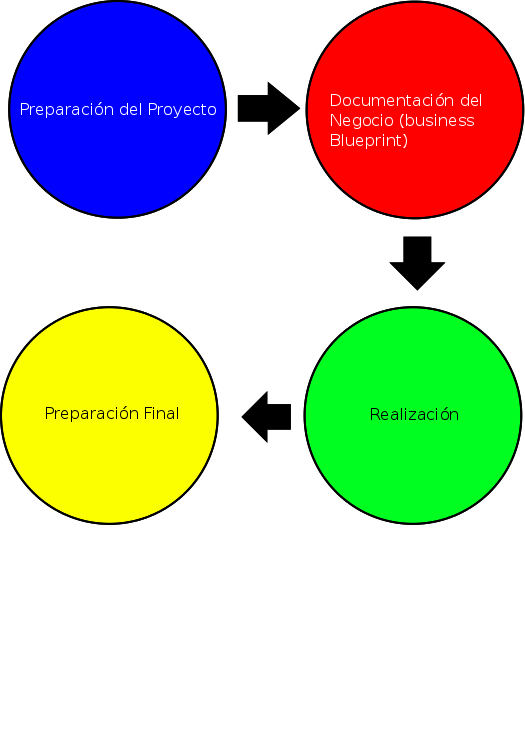
\includegraphics[scale=0.326,type=png,ext=.png,read=.png]{figures/RouteMap}
\caption{Mapa de Rutas usado en ASAP (Informaci'on obtenida en Waseen (2010) }
\label{fig:roadmap}
\end{figure}


\section{Fases de la metodolog'ia ASAP}
Seg'un Waseen (2010), esta metodolog'ia est'a dividida en 4 fases, las cu'ales se listan en los siguientes puntos.
\subsection{Fase 1: Preparaci'on Previa}
\indent Seg'un Khan (2002), en esta fase se evalúan dos factores cr'iticos del proyecto: en primer lugar la preparaci'on de la organizaci'on del mismo, ya que en este punto se realizan algunas tareas de gesti'on que son claves: Proveer un compromiso de la alta gerencia y apoyo, establecer metas y objetivos claros, acordar en los próximos pasos a dar dentro del proyecto, proveer un proceso eficiente de toma de decisiones, escoger un equipo que sea calificado y que represente las distintas 'areas funcionales.
\newline
\newline
\indent Seg'un Khan (2002), en segundo lugar, la planificaci'on del proyecto, ya que en este punto se deben identificar aquellos elementos que sean cr'iticos, dentro de los cuales se puede mencionar los que se listan a continuaci'on:
\begin{itemize}
\item Principios Rectores: Estos son principios de alto nivel que pueden ser establecidos al inicio del proyecto. Estos definen y comunican la visi'on de la empresa, ayuda a mantener el proyecto enfocado, y en el caso en que exista alg'un conflicto, sirve de base para su soluci'on. 
\item Principios estrat'egicos:  Estos son principios de negocio que direccionan las estrategias a utilizar. Al tener unas estrategias bien definidas, la implementaci'on se torna m'as f'acil, y as'i se pueden lograr los objetivos establecidos.
\item Impulsores del proyecto: Estos son los encargados de escoger el software ERP para una implementaci'on particular. Es importante recordar que SAP tiene distintas soluciones para ciertos tipos de empresas. 
\item Presupuestos, est'andares y indicadores: Al inicio del proyecto se debe establecer un presupuesto sobre el costo del mismo, adem'as que se deben definir los est'andares que va a utilizar y los distintos indicadores.
\end{itemize}
Seg'un Khan (2002), en tercer lugar, el equipo de implementaci'on, ya que es el responsable de que el proyecto se pueda llevar a cabo. Generalmente este equipo se encuentra integrado por consultores pertenecientes a organizaciones externas y por empleados internos de la compa\~n'ia. Este equipo est'a dividido en los siguientes grupos:
\begin{itemize}
\item Personal interno de la compa\~n'ia o Cliente.
\item Personal de Implementaci'on e Integraci'on: 'Este incluye a empleados de la empresa desarrolladora o de sub-contratistas.
\end{itemize}
El equipo de clientes est'a integrado por:
\begin{itemize}
\item Miembros del equipo central: Tienen dedicaci'on al 100\% del tiempo disponible dedicado al proyecto.
\item Equipo de extensi'on: Son los que tienen dedicaci'on del 20\%-50\% del tiempo al proyecto, dependiendo de la fase en la cual se encuentre.
\end{itemize}
\indent En este punto, los equipos definidos son organizados por los distintos m'odulos o funcionalidades.  
\newline
\newline
\indent Es fundamental que el equipo escogido tenga las siguientes capacidades:
\begin{itemize}
\item Analizar el impacto del nuevo sistema ERP sobre los procesos del negocio contra el proceso actual
\item Analizar los requerimientos funcionales y de implementaci'on. 
\item Dise\~nar un sistema integrado.
\item Proveer de conocimiento a los empleados durante el proyecto.
\end{itemize}
\subsection{Fase 2: Business Blueprint}
Seg'un Khan (2002), el objetivo principal de esta fase es comprender el funcionamiento actual de la empresa, para as'i poder determinar los requerimientos de implementaci'on basados en las necesidades que la organizaci'on pueda presentar en un futuro. Para esto, se realiza un an'alisis exhaustivo del negocio de la compa\~n'ia, c'omo se desenvuelve actualmente, e identificando las funcionalidades soportadas por el sistema actual. Luego son comparadas las pr'acticas existentes y sus funcionalidades  con las que son soportadas por SAP. 
\newline
\newline
\indent Seg'un khan (2002), durante esta fase, los ejecutivos y gerentes de la compa\~n'ia son entrevistados. Dichas entrevistas son realizadas dentro de grupos peque\~nos, o de manera individual. Luego, basado en las respuestas obtenidas, los consultores pueden entender y definir los siguientes par'ametros:
\begin{itemize}
\item El negocio de la compa\~nia
\item La forma de operar
\item Elementos cr'iticos del negocio
\item Procesos deseables a llevar a cabo en el negocio
\item Requerimientos del negocio y de funcionalidades
\item El alcance que tendr'a el proyecto
\item Los riesgos que posee el desarrollo del proyecto
\end{itemize}
Seg'un Khan (2002), al final de esta etapa es elaborado un documento llamado \textbf{Documento de Proyecto (Blueprint Document como se le conoce en ingl'es)}. 
Seg'un Khan (2002), este documento puede ser descrito como un modelo visual de la empresa. En este documento se detalla lo siguiente:
\begin{itemize}
\item Funcionalidad ya existente
\item Funcionalidad a desarrollar
\item Procesos actualmente en operacion
\item Alcance de la implementaci'on
\item Estructura organizacional
\item Funcionalidad diferida
\item Riesgos potenciales
\end{itemize}
\indent  Seg'un Khan (2002), una decisi'on fundamental que se toma en esta fase es la definici'on de una estructura organizacional SAP basada en los procesos de organizaci'on del negocio. 
\newline
\newline
\indent Seg'un Khan (2002), esta estructura determina c'omo los datos son definidos dentro del sistema, la complejidad de los datos de entrada, y el tama\~no de los archivos que contienen datos maestros. 
\newline
\newline
\indent Seg'un Khan (2002), la estructura definida debe haberse analizado bien en esta etapa, ya que cualquier cambio que fuera realizado en las fases siguientes, derivar'ia en un costo elevado.
\newline
\newline
\indent Seg'un Khan (2002), uno de los elementos m'as importantes de la estructura organizacional es el c'odigo que se le asigna a la compa\~n'ia, ya que este es el elemento m'as alto dentro de esta estructura armada. El c'odigo de la compa\~n'ia es una unidad legal y organizacionalmente independiente.Este representa a una unidad de contabilidad independiente, lo cual hace que posea sus propias componentes financieras.
\newline
\newline
\indent Seg'un Khan (2002), una de las partes de esta estructura es el \textbf{'Area de Control}. La misma simboliza a un elemento organizacional con la cual se manejan como estructura organizativa es la estructura del negocio. Esto no es m'as que la organizaci'on de la empresa en s'i. En otras palabras, las distintas 'areas funcionales, como Log'istica, Recursos Humanos, etc.
\subsection{Fase 3: Realizaci'on (Construcci'on y Pruebas)}
	Seg'un Khan (2002), durante esta fase, el sistema es configurado bas'andose en los requerimientos obtenidos en la fase anterior, y luego es probado. Esta fase no es r'igida, es decir, que la aplicaci'on de la misma es progresiva. En otras palabras, se construye, se prueba, se refinan los detalles y se vuelve a probar. En el Ap'endice A.3 se describen un poco las etapas por las cuales se pasa dentro de esta fase.

\subsection{Fase 4: Preparaci'on y Resultados Finales}
	Seg'un Khan (2002), en esta 'ultima fase hay varias tareas que deben ser llevadas a cabo para la culminaci'on de un proyecto realizado en SAP. Estas tareas son las que se listan a continuaci'on:
	
\begin{table}[H]
\footnotesize
\begin{tabular}{|l|l|}
\hline
\textbf{Tarea a Realizar}  & \textbf{Descripci'on}  \\
\hline
Refinar el Sistema creado & Una vez que se han realizado todas las pruebas al sistema y se haya recibido \\
                                        & la retroalimentaci'on del usuario final, se proceder'a a hacer las modificacio - \\
                                        & nes pertinentes para adaptar el sistema a los posibles cambios que puedan \\
                                        & surgir. Es posible que tanto las configuraciones, como las interfaces e amplia -\\
                                        & ciones tengan que sufrir alguna modificaci'on. \\
\hline
Planeacion de la preparaci'on & Este plan consiste en el conjunto de actividades que deben ser ejecutadas \\ 
de la Salida en Vivo                & las 'ultimas semanas antes de salir en vivo. Este 'ultimo t'ermino se refiere \\
                                              & a la ejecuci'on integral y puesta en producci'on de todo el sistema por parte\\
                                              & de los usuarios finales. \\
                                              & Este plan consiste en el conjunto de actividades que deben ser ejecutadas las\\
                                              & 'ultimas semanas antes de salir en vivo. Este 'ultimo t'ermino se refiere a la eje - \\
                                              & cuci'on integral y puesta en producci'on de todo el sistema por parte de los u- \\
                                              & suarios finales. \\
                                              & 	Algunas de estas actividades a realizar, son las que se listan a continuación: \\ 
											   & - Tareas variadas \\
											   & - Establecer un calendario y los hitos principales \\
											   & - Estimar tiempo de carga de datos por cada sub-carga \\
										       & - Asignaci'on de cada tarea a una persona \\
											   & - Establecer un per'iodo y el procedimiento para desconectar el sistema legal \\
											   &    previo. \\
											   & - Procedimiento de limpieza de datos \\
											   & \\
                                              & Este plan puede ser revisado por los gerentes del proyecto, los ejecutivos, equi -\\ 
                                              & po t'ecnico y l'ideres para su posterior aprobaci'on. \\
\hline
Entrenamiento del Usuario     & El autor se\~nala que una regla general que se deber'ia seguir en todo desarro- \\ 
Final                                       & llo en SAP es que el 10 \% de todo el tiempo invertido en el desarrollo deber'a \\ 
                                              & ser tomado para el entrenamiento. De este tiempo, al menos el 1\% deber'ia ser\\  
                                              &  tomado para el entrenamiento de los ejecutivos de la empresa. \\
                                              & El entrenamiento se hace necesario, ya que las personas que laboran en una empre- \\
                                              & sa ,por lo general realizan sus tareas diarias de una forma ya establecida. \\
\hline
Transferencia de Conoci -      & En este punto es importante que todos los conocimientos adquiridos por los con - \\ 
miento                                   & sultores durante el proceso del desarrollo del proyecto,  sean transmitidos a los \\ 
                                              & empleados de la compa\~n'ia, para que as'i, puedan replicar el sistema en otros \\ 
                                              & lugares. Ellos deben transmitirles los conocimientos acerca de SAP adicionalmente, \\ 
                                              & ya que los empleados en muchas ocasiones no tienen conocimiento acerca de este  \\
                                              &  tipo de tecnolog'ias. \\
\hline
Administraci'on del Sistema    & En este punto, el equipo encargado de realizar las pruebas al sistema y a los \\ 
                                              & servidores es el equipo de T'ecnicos (Basis). Aqu'i es donde se verifica si son \\
                                              & necesarios m'as servidores o m'as equipos de otro tipo. \\
\hline
Migraci'on de Datos                & En esta etapa se realiza la migraci'on de los datos restantes desde el sistema \\
                                               & existente al nuevo sistema creado en SAP. En este momento, el sistema anti - \\
                                               & guo permanece funcionando por un tiempo hasta que todos los datos migra - \\
                                               & dos sean validados. \\
\hline 
Pruebas Finales y Entona-       & En este punto se realizan pruebas de vol'umen y se procede  a colapsar el siste- \\
ci'on                                       & ma, para verificar que puede atender gran cantidad de solicitudes concurrentes, \\
                                              & y se realizan las modificaciones pertinentes. En este punto comienza la puesta \\
                                              & en vivo del sistema completo. \\
\hline
\end{tabular}
\caption{Tareas relacionadas con la Preparaci'on Final (Informaci'on obtenida en Khan (2002)}
\label{tb:asignaciones}
\end{table}

\section{Aplicaci'on para el Proyecto  de Pasant'ia}
Para este proyecto, se llegaron aplicar cada una de las fases de esta metodolog'ia, en su respectivo orden. 	
\newline
\newline	 
\indent En el pr'oximo cap'itulo se va a explicar el conjunto de actividades realizadas en las fases que formaron parte de este proyecto.